\subsection{具有无限状态的马氏链}

\begin{figure}[H]
    \centering
    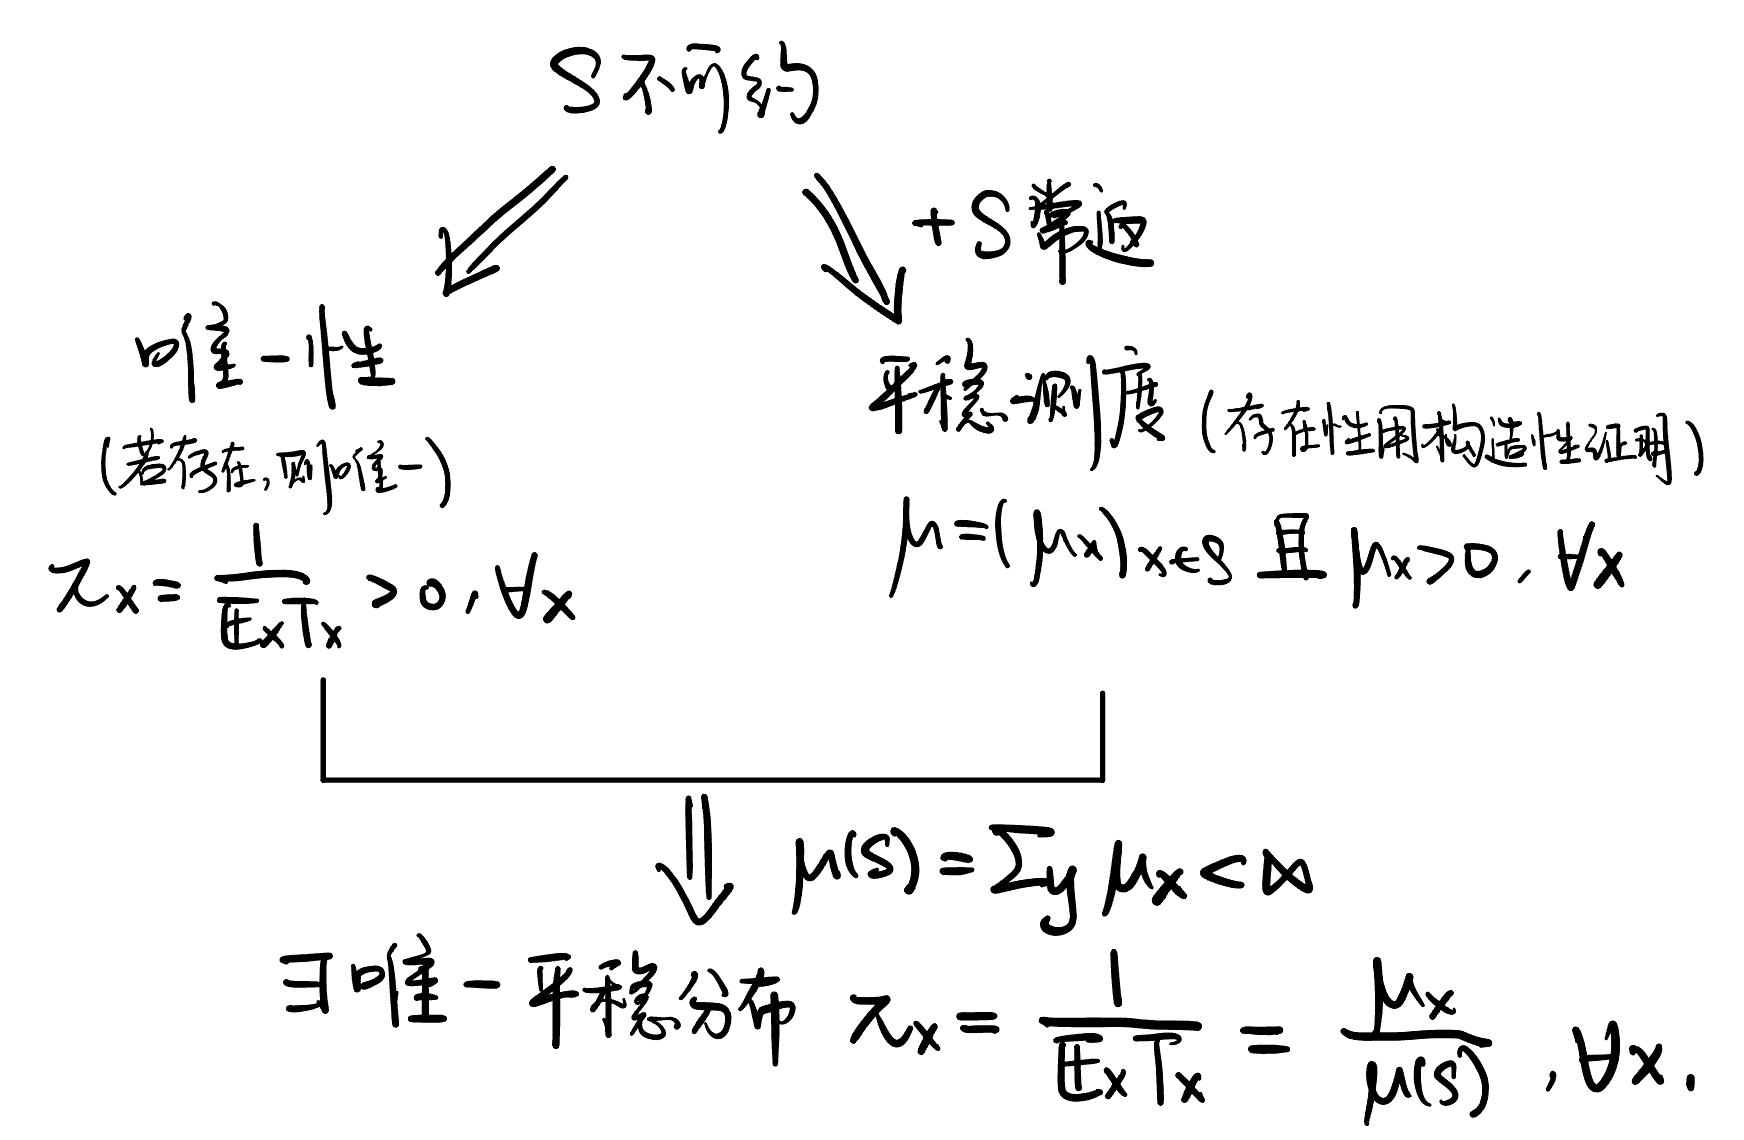
\includegraphics[width=0.65\textwidth]{figures/irreduce_summary.png}
    \caption{Summary}
\end{figure}

``构造性证明'' 见 \eqref{eq:stationary_measure}.

\begin{claim}
$S$ 不可约, 若存在平稳分布, 则 $\pi_x>0,\forall x\in S$.
\end{claim}

\begin{proof}
    设 $\exists x, \stt \pi_x=0$. $\pi=\pi P^n, \forall n\geq 0$. $\pi_x=\sum_y\pi_y p_{yx}^{(n)}, \forall n\geq 0$. $\Rightarrow \pi_y p_{yx}^{(n)}=0,\forall y\in S,n\geq 0$. 又因 $S$ 不可约, $\forall y\in S, y\to x$. 所以 $\exists n_y\geq 0, \stt p_{yx}^{(n_y)}>0$. $\Rightarrow \forall y\in S, \pi_y=0$. 这与 $\sum_y\pi_y=1$ 矛盾
\end{proof}

\begin{lemma}\label{lem:p84}
    $S$不可约, \framebox{若存在平稳测度 $\mu=(\mu_x)_{x\in S},\mu_x>0,\forall x$} (即``若 $S$ 常返成立''), \framebox{$\mu(S)=\sum_{x\in S}\mu_x<\infty$}, 则存在唯一平稳分布
    \begin{equation}
    \pi_x=\frac{1}{\EE_xT_x}=\frac{\mu_x}{\mu(S)}>0,\forall x
    \end{equation}
    注: $\pi_x=1/(\EE_xT_x)>0,\forall x$ 为必要条件

    $\Rightarrow \EE_xT_x<\infty, \forall x\Rightarrow \forall x$, $x$ 正常返 $\Rightarrow$ $S$正常返. (这是必要条件, 那反过来是否充分? 能否推出框内条件?)
\end{lemma}

$i \leftrightarrow j$, 则由 Cor \ref{cor:trans_recurrent}, $i$正常返 $\iff$ $j$正常返, $i$零常返 $\iff$ $j$零常返, $i$非周期 $\iff$ $j$非周期. $p_{jj}>0\Rightarrow d(j)=1$. 

\begin{theorem}
    $S$ 不可约, 则下列结论等价
    \begin{enumerate}
        \item 某个状态正常返
        \item 存在平稳分布 $\pi$
        \item 所有状态正常返
    \end{enumerate}
\end{theorem}

\begin{proof}
    $(3)\Rightarrow (1)$ 显然, $(2)\Rightarrow (3)$ 在上面注记中已证. 要证 $(1)\Rightarrow (2)$.

    $S$不可约, 存在$x$正常返 $\Rightarrow$ $S$不可约, 常返. 由 Thm \ref{thm:stationary_exists_unique} 及 \eqref{eq:stationary_measure}, 存在平稳测度 $\mu_y=\sum_{n\geq 0}\PP_x(T_x>n,X_n=y),\forall y\in S$. 由 Lem \ref{lem:p84} 框内条件知, 平稳测度要求 $\mu(S)<\infty$.
    \[
    \begin{aligned}
        \mu(S) = \sum_{y\in S}\mu_y
        &=\sum_{n\geq 0}\sum_{y\in S}\PP_x(T_x>n,X_n=y)\\
        &=\sum_{n\geq 0}\PP_x(T_x>n)=\EE_x T_x<\infty
    \end{aligned}
    \]
    注: $T_x=\sum_{n\geq 0}\II_{\{T_x>n\}}=\sum_{n\geq 1}\II_{\{T_x\geq n\}}$.

    存在平稳分布 $\pi_x=\mu_x/\mu(S)>0,\forall x$.
\end{proof}

\begin{corollary}
    对不可约链, 下列情况之一必发生
    \begin{enumerate}
        \item $S$非常返, 则不存在平稳分布
        \item $S$常返, 则对 $\forall x\in S$, 存在平稳测度 $\mu^{(x)}=(\mu_y^{(x)})_{y\in S}$. (由 Thm \ref{thm:stationary_exists_unique} 定义).
        \begin{enumerate}
            \item $\forall x,\mu^{(x)}(S)=\EE_xT_x<\infty$, 则$S$正常返, 则存在唯一平稳分布
            \item $\forall x,\mu^{(x)}(S)=\EE_xT_x=\infty$, 则$S$零常返, 则不存在平稳分布
        \end{enumerate}
    \end{enumerate}
\end{corollary}

\subsubsection{广义生灭链}

\begin{example}[带反射壁的随机游动(Durrett 1.54)]
    质点在 $S=\{0,1,2,\cdots\}$ 移动, 规定
    \begin{figure}[H]
        \centering
        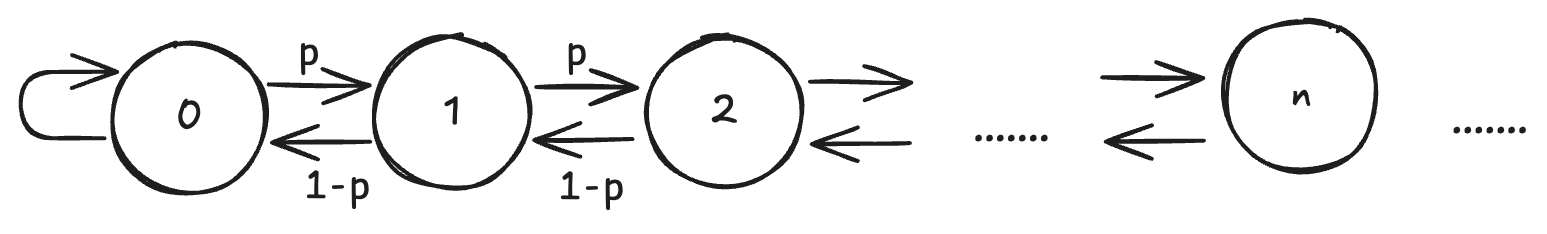
\includegraphics[width=0.65\textwidth]{figures/g_birth_death.png}
    \end{figure}
    $p\in (0,1)$, $X_n$: 表示 $n$ 时刻质点所在位置. 则
    \begin{enumerate}
        \item $p\in (0,1/2)$ 时, 存在唯一平稳分布, $S$ 正常返
        \item $p>1/2$ 时, $S$ 非常返, 不存在平稳分布
        \item $p=1/2$ 时, $S$ 零常返, 不存在平稳分布
    \end{enumerate}
\end{example}

\begin{proof}
\begin{enumerate}
    \item (Step 1) $S$不可约, 则平稳分布若存在则唯一
    
    (Step 2) (存在性) 回顾 Exa \ref{exa:birth_death}, 与当前例子的区别是状态空间 $S$ 是否有限. 设 $\pi$ 满足DBC, $\pi_xp_{xy}=\pi_yp_{yx},\forall x,y$. $\pi_ip_{i,i+1}=\pi_{i+1}p_{i+1,i},\forall i\geq 0$. $\pi_i p=\pi_{i+1}(1-p),\forall i\geq 0$.
    \[
    \pi_{i+1}=\frac{p}{1-p}\pi_i=\left(\frac{p}{1-p}\right)^{i+1}\pi_0,\forall i\geq 0
    \]
    \[
    \pi_i=\left(\frac{p}{1-p}\right)^{i}\pi_0,\forall i\geq 0\tag{*}
    \]
    又由 $\sum_i \pi_i=1$, 有
    \[
    1=\pi_0\sum_{i\geq 0}\left(\frac{p}{1-p}\right)^i=\pi_0\frac{1}{1-\frac{p}{1-p}}\Rightarrow \pi_0=\frac{1-2p}{1-p}\in (0,1)
    \]
    代回 $(*)$, 得 $\pi_i>0,\forall i$. 其中无穷级数 $\sum_{i\geq 0}\left(\frac{p}{1-p}\right)^i$ 当 $|p/(1-p)|<1$ 时收敛, 即 $p<1/2$ 时. ($\sum_{i=0}^{\infty}r^i=1/(1-r), \forall |r|<1$)
    \item 只需证状态 $0$ 暂留, 又因为 $0\to 1$, Lem \ref{lem:commu_recurrent}, 故只需证 $1>\rho_{1,0}=\PP_1(T_0<\infty)=\PP_1(V_0<\infty)$. 考察 $\PP_x(V_0<\infty)$. 注意到
    \[
    \{V_0<\infty,X_0=x\neq 0\}=\bigcup_{M\geq 0}\{V_0=M,X_0=x\neq 0\}=\bigcup_{M\geq 0}\bigcup_{N\geq x+M}\{V_0<V_N,X_0=x\neq 0\}
    \]
    $X_0=x\neq 0, \forall N\geq x+M+10000000$, $M=V_0<V_N<V_{N+1}$.

    令 $h(x):=\PP_x(V_0<V_N)$, 则
    \[
    \begin{cases}
        h(0)=1,h(N)=0\\
        h(x)=ph(x+1)+(1-p)h(x-1) & \forall x\neq 0,N
    \end{cases}
    \]
    由 Exa \ref{exa:1.43}, $\theta=(1-p)/p<1$ 时, $h(x)=(\theta^x-\theta^N)/(1-\theta^N),\forall x\in S$.
    \item 考虑一步转移情况.
    \[
    \begin{aligned}
        \EE_0T_0 &= \EE_0[T_0\II_{\{X_1=0\}}]+\EE_0[T_0\II_{\{X_1=1\}}]\\
        &=\EE_0[T_0|X_1=0]p_{0,0}+\EE_0[T_0|X_1=1]p_{0,1}\\
        &\xlongequal{\text{Markov}}\EE[V_0+1|X_0=0]\frac{1}{2}+\EE[V_0+1|X_0=1]\frac{1}{2}\\
        &=\frac{1}{2}(\EE_0(1)+\EE_1(1))+\frac{1}{2}\EE_1V_0\\
        &=1+\frac{1}{2}\EE_1V_0
    \end{aligned}
    \tag{*}
    \]
    考察 $g(x)=\EE_xV_0$.

    (Step 1) 考察 $\EE_x(V_0\land V_N)$, 同 Exa \ref{exa:1.48} 类似计算得到 $\EE_x(V_0\land V_N)=x(N-x)$.

    (Step 2) $\EE_1V_0\geq \EE_1(V_0\land V_N)=N-1\to +\infty, (N\to +\infty)$. 代回 $(*)$ 得 $\EE_0T_0=+\infty$
\end{enumerate}
\end{proof}
\newpage